%Dumb approach: explore all timings T for each subset of $E_L$.
%
%Slightly smarter approach:
%\begin{outline}
%  \1 apply delta debugging to efficiently search subsets of $E_L$
%  \1 But $T$ is still really important to get right. We tried a replay algorithm that just maintained relative spacing between inputs, but it didn't work.
%  \1 Problem is that internal events matter. We need to maintain causal relationships.
%  \1 But we're  changing history, i.e. the original causal relation is changing
%  \1 so we define equivalence to reason about changes to history
%  \1 we also need to time out on missing internal events.
%  \1 and let unexpected events through
%  \1 this leaves exactly one set of timings $T$ to look at, that in our experience reliably reproduces the bugs while still minimizing.
%\end{outline}
%
%In the next section we outline our solution to these difficulties.
% -------

To make the discussion concrete we describe a
documented bug\footnote{Now fixed, as we have heard.} in the Floodlight
open source control platform~\cite{floodlight_bug}. Floodlight is distributed across
multiple controllers for high availability, and provides support for
virtualization. Switches maintain one hot connection to a master controller and
several cold connections to replica controllers. The \emph{master} holds the
authority to modify the configuration of switches, while the other
controllers are in \emph{backup} mode and do not perform any changes to the
switch configurations unless they detect that the master has crashed.

\begin{figure}[t]
  %\hspace{-10pt}
  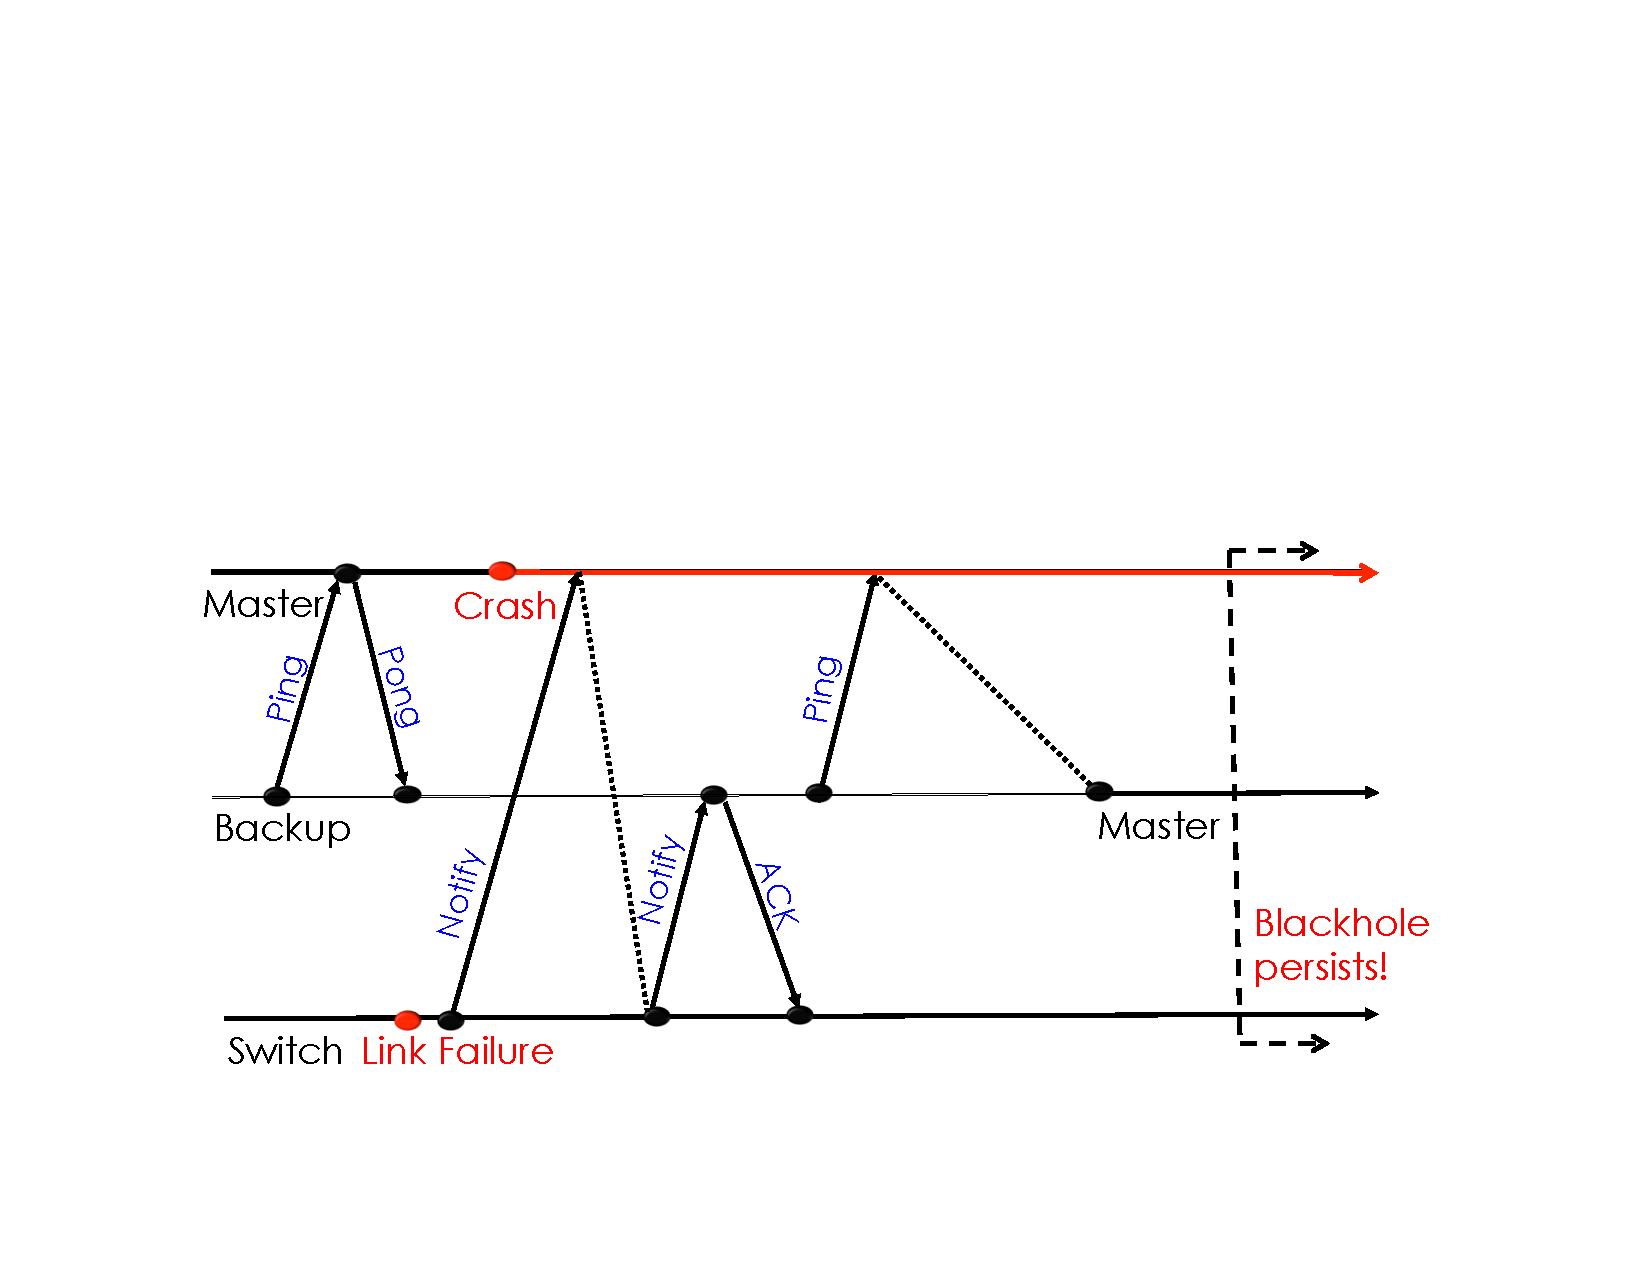
\includegraphics[width=3.25in]{../diagrams/case_study/example_bug.pdf}
  \caption[]{\label{fig:example} Floodlight failover bug. External inputs
             are depicted as red dots, internal events are depicted as black
             dots, and the dotted message line depicts a timeout.}
\end{figure}

The failover logic in Floodlight is not implemented correctly, leading to the
following race condition depicted in
Figure~\ref{fig:example}:
a link fails (E1), and the switch attempts to notify the controllers (E2,E4) shortly after the master
controller has died (E3), but before a new master has been selected (E6). In this case, all live controllers are in
the backup role and will not take responsibility for updating the switch
flow table (E5). At some point, a backup notices the master failure and
elevates itself to the master role (E6). The new master will proceed to manage
the switch, but without ever clearing the routing entries for
the failed link (resulting in a persistent blackhole).

There were only two external inputs (E1,E3) shown in our example.
However, a developer or operator encountering this bug in practice would not be
given this concise version of events. Instead, the trace would likely contain a wealth
of extraneous inputs, making it difficult
to reason about the underlying root cause;
%In the worst scenario, operators may need to examine logs from a production
%network, which contain a substantial number of hardware failures, topology changes,
%and other potential triggering events,
%all of which may appear characteristic of normal operating
%conditions at first glance;
assuming 8.5 network error events per
minute~\cite{Greenberg:2009:VSF:1592568.1592576} and 500 VM migrations per
hour~\cite{Soundararajan:2010:CBS:1899928.1899941},
there would be at least $8.5 \cdot 60 + 500 \approx 1000$ inputs reflected in
an hour-long trace. Yet despite the large number of events reflected in the
log, many bugs encountered in practice are triggered by a
relatively small number of events (as we show in \S\ref{sec:casestudies}).

Going back to our example,
suppose a log of this execution includes many more (extraneous) inputs. If we
were to remove an
extraneous event, the blackhole would still persist after replaying.
When we prune the controller crash though, the blackhole will be resolved properly, and
when we prune the link failure, no blackhole will occur. The MCS
of the log is therefore the conjunction of the controller crash and the link
failure, along with their timing depicted in Figure~\ref{fig:example}.

\subsection{Searching for Subsequences}
\label{subsec:algorithm}

Given a log $(E_L, T_L, C_L)$ exhibiting an invariant violation,
our goal is to identify its MCS. In a brute force fashion,
the most obvious way to do so involves exploring all timings $T$ for each
subsequence of $E_L$, feeding each one to a replay mechanism (which we
describe in \S\ref{sec:systems_challenges}) and checking whether the bug
persists. Yet this approach is clearly intractable, so we seek a more efficient
means.

We find a more efficient algorithm for searching subsequences of $E_L$ from
the software engineering community: the original formulation of delta debugging~\cite{Zeller:1999:YMP:318773.318946}
takes a single input (\eg~an HTML page)
for a non-distributed program (\eg~Firefox), and performs a divide-and-conquer
search, repeatedly runs the program on subsets of the input
until finding a minimal subset (\eg~a single tag) that is sufficient
for triggering a known bug. Specifically, delta debugging finds a locally minimal
causal sequence~\cite{Zeller:1999:YMP:318773.318946},
meaning that if any input from the sequence is pruned, no invariant violation
occurs. We can similarly explore subsequences of $E_L$ by letting delta
debugging iteratively select subsequences and replaying each subsequence with
some timing $T$ to test whether the bug persists.
The delta debugging algorithm is shown in
Figure~\ref{fig:ddmin} (with `$test$' replaced by `$replay$').

\begin{figure*}[t]
\caption{Automated Delta Debugging Algorithm From~\cite{Zeller:1999:YMP:318773.318946}}
\begin{boxedminipage}{\textwidth}
Input: $\cfail$ s.t. $\cfail$ is a trace and $\test(\cfail) = \DFAIL$. Output: $\dfail
= \ddmin(\cfail)$ s.t. $\dfail \subseteq
\cfail$, $\test(\dfail) = \DFAIL$, and~$\dfail$ is minimal.
\begin{align*}
\ddmin(\cfail) &= \ddmin_2(\cfail, \emptyset) \quad \text{where} \\
\ddmin_2(\dfail, R) &=
\begin{cases}
\dfail & \text{\hphantom{else }if $|\dfail| = 1$ (``base case'')} \\
\ddmin_2\bigl(\done, R\bigr) &
\text{else if $\test(\done \cup R) = \DFAIL$ (``in $\done$'')} \\
\ddmin_2\bigl(\dtwo, R\bigr) &
\text{else if $\test(\dtwo \cup R) = \DFAIL$ (``in $\dtwo$'')} \\
\ddmin_2\bigl(\done, \dtwo \cup R\bigr) \cup \ddmin_2\bigl(\dtwo, \done \cup
R\bigr) & \text{otherwise (``interference'')}
\end{cases}
\end{align*}
\begin{center}
where $\test(T)$ denotes the state of the system after executing the trace $T$,
$\DFAIL$ denotes a invariant violation, \\
$\done \subset \dfail$, $\dtwo \subset \dfail$, $\done \cup \dtwo = \dfail$, $\done \cap
\dtwo = \emptyset$, and $|\done| \approx |\dtwo| \approx |\dfail| / 2$
hold.
\end{center}
\end{boxedminipage}
\label{fig:ddmin}
\end{figure*}

\eat{ % Original O(n^2) algorithm
\begin{figure*}[t]
\caption{Minimizing Delta Debugging Algorithm From~\cite{Zeller:2002:SIF:506201.506206}}
\begin{boxedminipage}{\textwidth}
Input: $\cfail$ s.t. $\cfail$ is a trace and $\test(\cfail) = \FAIL$. Output: $\dfail
= \ddmin(\cfail)$ s.t. $\dfail \subseteq
\cfail$, $\test(\dfail) = \FAIL$, and~$\dfail$ is 1-minimal.
\begin{align*}
\ddmin(\cfail) &= \ddmin_2(\cfail, 2) \quad \text{where} \\
\ddmin_2(\dfail, n) &= 
\begin{cases}
\ddmin_2(\Delta_i, 2) & \text{\hphantom{else }if $\exists i \in \{1, \dots, n\} \cdot \test(\Delta_i) = \FAIL$ (``reduce to subset'')} \\
\ddmin_2\bigl(\nabla_i, \max(n - 1, 2)\bigr) & 
\text{else if $\exists i \in \{1, \dots, n\} \cdot \test(\nabla_i) = \FAIL$ (``reduce to complement'')} \\
\ddmin_2\bigl(\dfail, \min(|\dfail|, 2n)\bigr) & \text{else if $n < |\dfail|$ (``increase granularity'')} \\
\dfail & \text{otherwise (``done'').}
\end{cases}
\end{align*}
where $\test(T)$ denotes the state of the system after executing the trace $T$,
$\FAIL$ denotes a invariant violation, \\
$\nabla_i = \dfail - \Delta_i$, $\dfail = \Delta_1 \cup \Delta_2 \cup \dots \cup \Delta_n$, all
$\Delta_i$ are pairwise disjoint sequences of inputs, and $\forall \Delta_i \cdot |\Delta_i| \approx |\dfail| / n$
holds.
\end{boxedminipage}
\label{fig:ddmin}
\end{figure*}
}

\eat{
As we will see though, our problem differs from the original formulation of delta debugging in two dimensions.
First, delta debugging assumes that input is inserted at a single point in
time. In contrast, input to SDN controllers includes many messages spread
throughout time.
Second, delta debugging assumes a single program under test. Our input depends on
causal relationships across
concurrently running nodes.

For the purposes of this section, we model our problem as follows.
We are given a single, globally ordered trace of events that ends in
a invariant violation, and we return a minimal causal subsequence
of the trace. The trace includes input events
(\eg~link failures), control message sends and receipts between
switches and controllers,
and internal state changes (\eg~the
backup deciding to elevate itself to master in the Floodlight case) labeled
with the control process that made the state change.
In \S\ref{subsec:exploration}, we describe how we obtain the globally
ordered trace in practice.

In the rest of this section we describe how we
replay inputs to control software and
cope with alterations to the causal history of an execution.
}

\subsection{Searching for Timings}
\label{subsec:replay}

% Needs a back pointer. "Once a subsequence has been chosen,"...
Even with an algorithm for systematically exploring subsequences of $E_L$, the
timing of those subsequences during replay is crucial for reliably
reproducing the
invariant violation throughout the delta debugging execution. Na\"ively injecting inputs often fails to
trigger the original invariant violation, even without having pruned any
events. In particular, we tried and failed to reproduce errors when scheduling inputs
with the following simple algorithm:
\begin{align*}
t'_0 = 0 \\
t'_i = t'_{i-1} + |t_{i} - t_{i-1}|
\end{align*}
where $t'_i$ is the simulation's clock value when it injects the $i^{th}$ input, and $t_i$ is
the timestamp of the $i^{th}$ input from the original run. In other words, simply
maintaining the relative timing between inputs is not sufficient.

The problem with the simple scheduling algorithm is that it does not take into
account events that are internal to the control software, such as
message receipts, timers going off, or internal state
changes like the backup node in the Floodlight example deciding to elevate
itself to master; if the ordering of inputs and internal events is
perturbed, the final output may differ.
Consider for example that if a controller's garbage collector happens to run
while we replay inputs, it may delay an internal state transition until
after the simulator injects an input that depended on it in the original run.

Our challenge is to maintain causal relationships.
Formally, to reliably reproduce the original invariant violation
we need to
inject an external input $e$ at exactly the point when all other
events (both external and internal) that precede it in the happens-before
relation ($\{i \mid i \rightarrow e\}$) from the original execution have
occurred~\cite{tel2000introduction}.

\eat{
\colin{Somewhat redundant. Maybe wait until use cases.}
While the inputs and original internal events are given to us,
we become aware of new internal events throughout replay by
(i) monitoring
control message receipts between controllers and switches,
and (ii) interposing on the controllers' logging library and notifying the
simulator whenever the control software executes a log statement (which serve to mark relevant state
transitions). Note that to achieve truly deterministic
replay, these log statements would need to
be highly granular, capturing information such as thread scheduling decisions;
we show in \S\ref{subsec:case_studies}
however that pre-existing, course granular log statements are often sufficient to
successfully reproduce bugs.
}
%\footnote{We discuss this problem further in
%\S\ref{subsec:domain_knowledge}.}
%Note that the developer must provide enough logging statements
%so that relevant internal state changes are captured and visible to our
%tool.

\subsection{Functional Equivalence}
\label{subsec:functional_equivalence}

Replay is made substantially more complicated by the fact
that the delta debugging algorithm is pruning inputs from the history of the
execution, thereby changing the resulting internal events generated by the control
software. In particular, internal events may differ syntactically (\eg~sequence numbers
of control packets may all differ), old internal events from the original
execution may not occur after pruning, and new internal events that were not
observed at all in the original execution may appear.

We observe that many internal events are {\em functionally
equivalent}, in the sense that they
have the same effect on the state of the system with respect to triggering the
invariant violation (despite syntactic differences). For example, flow
modification messages may cause switches to make the same change to their forwarding behavior
even if the transaction identifier of the messages differ.

We leverage this observation by defining
domain-specific masks over semantically extraneous fields of
internal events.\footnote{One consequence
of applying masks is that bugs involving masked fields are outside the purview of
\simulator.} We show four examples of masked values
in Table~\ref{tab:fingerprints}.

These masks define equivalence classes
of internal events. Formally, we consider an internal event $i'$ observed in an altered trace
equivalent to an internal event $i$ from the original trace iff all unmasked
fields have the same value
and $i$ occurs between $i'$'s preceding and succeeding inputs in the
happens-before relation.

\eat{
\begin{figure}[t]
    %\hspace{-10pt}
    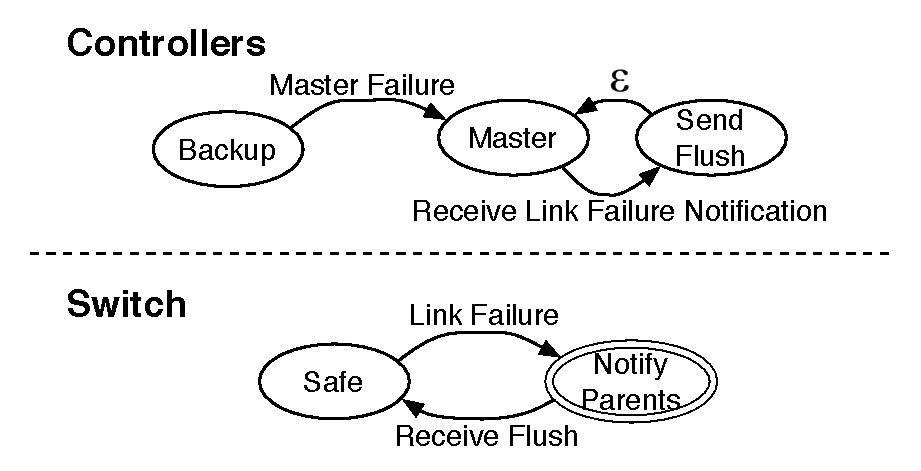
\includegraphics[width=3.25in]{../diagrams/state_machines/controller_switch.pdf}
    \caption[]{\label{fig:state_machines} Simplified state machines for the switch and
    controllers in the example Floodlight bug. Double outlined states
    represent presence of the blackhole.}
\end{figure}
}

\begin{table}
\centering
\begin{tabular}{|l|l|}
\hline
Internal message & Masked values \\
\hline
OpenFlow headers & transaction id\\
OpenFlow FLOW\_MODs & cookie, buffer id \\
Log statements & varargs parameters to printf \\
\hline
\end{tabular}
\caption{Example internal messages and their masked values. The masks serve to
define equivalence classes.}
\label{tab:fingerprints}
\end{table}

\subsection{Handling Absent Internal Events}
\label{subsec:divergence}

Given an equivalence relation over internal events, replay
is responsible for maintaining equivalent happens-before constraints from the
original execution.
But syntactic differences are not the
only possible change induced by pruning: internal events
may also cease to appear.

\eat{
The structure of the control
software's state machine (which we do not assume to know) determines whether
internal events disappear. Consider the simplified state machines for the switch and
controllers from the Floodlight case shown in
Figure~\ref{fig:state_machines}. If we prune the link failure input, the
master will never receive a link failure notification and
transition to and from `Send Flush'.
}

To ensure that delta-debugging finds minimal causal sequences that do not contain those
absent internal events, we proceed with replay.
Specifically, our approach is to wait for expected equivalent internal events, but time out and proceed
if they do not occur within a certain time \textepsilon.

In most cases this approach successfully reproduces the original invariant
violation, assuming \textepsilon~is larger than variations in execution speeds
between internal events. If the value of \textepsilon~is too large, however, we may end up
waiting too long for the happens-before predecessors of an input $e_i$ such that a
successor of $e_i$ occurs before we have injected $e_i$,
thereby violating causality.
% \sam{Is it worth noting that this isn't necessarily a problem? If a successor occurs, it means it wasn't causally related to $e_i$, but the ordering still might matter for further successors.}

If the event scheduling algorithm detects that it has waited too long, it
replays the trace from the beginning up until the immediately prior input,\footnote{An alternative
would be to take a snapshot of the controllers' state at every injected input
and start from the latest snapshot.} this time
knowing exactly which internal events in the current input interval are
and are not going to occur before injecting the next input. We show the overall event scheduling algorithm
in Figure~\ref{fig:peek}.

\begin{figure}
  \begin{pseudocode}[framebox]{CausalInference}{events}
    \PROCEDURE{Replay}{subsequence}
    \FOR e\textsubscript{i}\ in\ subsequence \\
    \BEGIN
    \IF e\textsubscript{i}\ is\ an\ internal\ event \\
    \AND e\textsubscript{i}\ is\ not\ marked\ absent:
    \THEN
    \BEGIN
      \Delta \GETS |e\textsubscript{i}.time - e\textsubscript{i-1}.time| + \epsilon \\
      wait\ up\ to\ \Delta\ seconds\ for\ e\textsubscript{i} \\
      \IF e\textsubscript{i}\ did\ not\ occur:
      \THEN mark\ e\textsubscript{i}\ as\ absent
    \END
    \ELSEIF e\textsubscript{i}\ is\ an\ input:
    \THEN
    \BEGIN
      \IF a\ successor\ of\ e\textsubscript{i}\ occurred: \\
      \INLINECOMMENT{waited too long}
      \THEN
        \RETURN{\CALL{Replay}{subsequence}}
      \ELSE
        inject\ e\textsubscript{i}
      \END
    \END
    \ENDPROCEDURE
    \COMMENT{See Figure~\ref{fig:ddmin} for invocation} \\
  \end{pseudocode}
  \label{fig:peek}
  \caption{{\tt Replay} is responsible for replaying subsequences of events
  chosen by delta debugging (Figure~\ref{fig:ddmin}) and determining
  if the bug reappears. \colin{Fix framebox width}}
\end{figure}

%\begin{figure}
%\begin{boxedminipage}{\linewidth}
%\begin{Verbatim}[commandchars=\\\{\}]
%subsequence = [e\textsubscript{1}, e\textsubscript{2}, ..., e\textsubscript{j}]
%// e\textsubscript{1} is always an input
%
%function replay(subsequence):
%  bootstrap the simulation
%  for e\textsubscript{i} in subsequence:
%    if e\textsubscript{i} is an internal event and
%          e\textsubscript{i} is not marked absent:
%      \textDelta = |e\textsubscript{i}.time - e\textsubscript{i-1}.time| + \textepsilon
%      wait up to \textDelta seconds for e\textsubscript{i}
%      if e\textsubscript{i} did not occur:
%        mark e\textsubscript{i} absent
%    else if e\textsubscript{i} is an input:
%      if a successor of e\textsubscript{i} occurred:
%        // waited too long
%        return replay(subsequence)
%      else:
%        inject e\textsubscript{i}
%\end{Verbatim}
%\end{boxedminipage}
%\end{figure}

\subsection{Handling New Internal Events}
\label{subsec:new_events}

The last possible change induced by input pruning is the occurrence of new
internal events that were not observed in the original trace.
New events ultimately leave open multiple possibilities for where
we should inject the next input. Consider the following case:
if $i_2$ and $i_3$ are internal events observed
during replay that are both in the same equivalence class as a single event $i_1$ from the
original run, we could inject the next input after $i_2$ or after $i_3$.

% TODO: figure this figure out
%\begin{wrapfigure}{c}{1.3\linewidth}
%  \centering
%  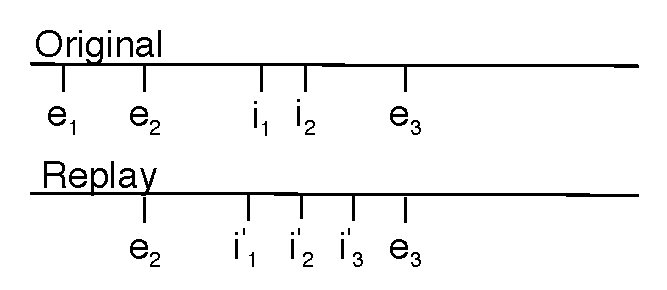
\includegraphics[width=\linewidth,height=0.8in]{../diagrams/state_machines/event_sequence.pdf}
%\end{wrapfigure}

In the general case it is always possible to construct two state machines that lead
to differing outcomes: one that only leads to the invariant violation when
we inject the next input
before a new internal event, and one that only leads to the
invariant violation when we inject the next input after a new internal
event. In other words, to be guaranteed to traverse any existing suffix that leads
to the invariant violation, it is necessary to recursively branch, trying both
possibilities for every new internal event. This implies an exponential number of
possibilities to be explored in the worst case.

Exponential search is not a practical option. Our heuristic when waiting for expected internal
events is to proceed normally if there are intermediate new internal events,
always injecting the next input when its last expected predecessor
either occurs or times out. This ensures that we always find suffixes that
contain only a subset of the (equivalent) original internal events, but leaves open the
possibility of finding divergent suffixes that still lead to the invariant
violation. This is reasonable because not even branching on new
internal events is guaranteed to find the globally shortest fault-inducing input
sequence:
there may be other unknown
paths through the state machine leading to the invariant violation that are
completely disjoint from the original execution.

Luckily, crucially ambiguous new internal events are not problematic for the
control software we evaluated, as we show in \S\ref{subsec:case_studies}.
We conjecture that ambiguous new internal events are
rare because SDN software is a control plane system,
and is designed to quiesce quickly (\ie~take a small number of internal
transitions after any input event, and stop at highly connected vertices).
Concretely, SDN programs are often structured as (mostly independent) event
handlers, meaning that pruning input events simply triggers a subset of the original
event handlers.
\eat{
As an illustration, consider the state machines
in Figure~\ref{fig:state_machines}:
the controllers quickly converge to a single state (either ``Master'' or
``Backup''), as do the switches (``Safe'').
}

In the next section we describe some
of the practical challenges we have overcome to realize our approach.
We have ultimately found with our system that applying delta debugging to explore
subsequences of $E_L$ and striving to ensure that our timing $T$ maintains
causal dependencies reliably finds small MCSs.

